\section{乘除法指令的添加}\label{s: lab3}

\foreword{
    记忆的永恒
}{
    萨尔瓦多·达利
}{
    时间是不断运动的永恒影像。
    %    人们应该始终把自己看作第二天就要死亡的人。将您扼杀的就是您以为面前还有无尽的时间。
}{
    Figures/C3.jpg
}

关于乘除法指令,在上学期的计组实验中已经有过初步的了解,但是当时直接使用了``*''与``/''直接实现,

关于 ``*'' 运算符,对于 Artix-7 系列的 FPGA,目前 Vivado 实现 ``*'' 运算符时会默认采用 DSP48 器件
(内含固化的 16 位乘法器电路),所以最终实现的电路的时序通常不错,
也几乎不消耗 LUT 资源。采用这种方式推导出的乘法器电路有两个 32 位数输入、
一个 64 位输出,具有单周期延迟,即输入数据之后当拍就能输出结果。

关于``/''和``\%'',我们这里禁止直接使用完成乘除法的运算,其主要的原因是如果直接使用这类运算符的话,
Vivado的综合工具将实现出一个用LUT实现的单周期除法运算部件,时序会非常非常非常的差。

在这里我们给出大家两种关于乘除法指令实现的方法。

\subsection{运用Xilinx IP的方法}

对于乘法运算部件,根据上面所述,直接使用运算符实现即可。

对于除法运算部件,这里调用IP核实现,在工程栏的``IP Catalog''中,
然后搜索``Divider Generator'',进入除法器的配置页面,在下面我们给出一点关于除法器配置的建议:

\begin{itemize}
    \item 建议采用Radix2算法,它的优点是消耗的资源少,缺点是完成运算需要的迭代周期数较多。
    \item 需要实现有符号除和无符号除,建议定义两个除法器IP。
    \item 将Remainder Type选择为Remainder,确保余数的类型为整数型。不需要除0检测
    \item AXI接口的流控这里可以选择Non Blocking
    \subitem 
    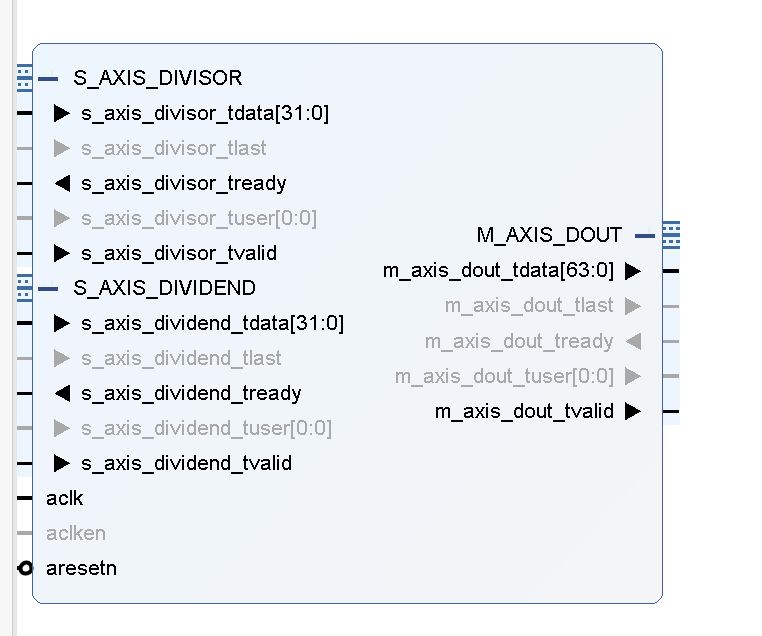
\includegraphics[width=0.6\linewidth]{Figures/fig1.png}
    \item \texttt{s\_axis\_dividend\_tdata} 对应计算时输入的被除数数据,\texttt{s\_axis\_divisor\_tdata} 对应计算时输入的除数数据,\texttt{m\_axis\_dout\_tdata} 中输出得到的商和余数,[63:32]位存放商,[31:0]存放余数。
    (上图中其他使用的信号,可能大家并不会完全用到,请根据自身使用情况进行调整,不需要跟途中的除法器配置完全保证一致,只需要保证功能可以正常实现即可)
\end{itemize}

对于两个输入通道和一个输出通道,除了有上述的数据信号外,每个通道都有一对 tvalid、
tready 信号。这是一对 “握手” 控制信号,其工作原理类似于我们在 CPU 流水线之间使用的
valid、allowin 信号。tvalid 是请求信号,tready 是应答信号。在时钟上升沿到来时,如果采样得
到 tvalid 和 tready 都等于 1,则请求发起方和接收方之间完成一次成功的握手。如果我们假想接收方有一组触发器缓存,那么所谓的成功握手是指发送方的数据写入接收方的缓存中,也就是在
握手成功的这个上升沿之后,触发器缓存会变为发送方的数据。

我们假设在执行流水阶段调用所生成的除法器 IP。在除法指令处于执行流水级且没有
对除法器成功输入数据的时候,同时将
\texttt{s\_axis\_dividend\_tvalid}和\texttt{s\_axis\_divisor\_tvalid}
置为 1。当发现 \texttt{s\_axis\_dividend\_tready} 和 \texttt{s\_axis\_divisor\_tready} 反馈为 1 后(此时在一
个时钟上升沿同时看到 tvalid 和 tready 为 1,表示握手成功),需要将 \texttt{s\_axis\_dividend\_tvalid} 和
\texttt{s\_axis\_divisor\_tvalid} 清 0,也就是确保握手成功的那个时钟上升沿之后的 \texttt{s\_axis\_dividend\_tvalid}
一定同时置为 1,那么这里生成的除法器 IP 反馈的 \texttt{s\_axis\_dividend\_tready} 和 \texttt{s\_axis\_divisor\_tready}
一定也同时置为 1。这里再次强调,被除数和除数输入的 tready 置起后(也就是握手成功后),
tvalid 一定要撤销,否则对于除法器 IP 来说,它会认为又有一个新的除法运算。

完成输入数据的握手之后,除法指令就需要在执行流水级等待除法器 IP 最终输出结果。当
\texttt{m\_axis\_dout\_tvalid} 置为 1 时,表示除法计算完成。此时除法指令就可以从 \texttt{m\_axis\_dout\_tdata}
上取出计算结果,进入流水线的后续阶段。由于前面我们将流控策略设置为 Non Blocking,因此
输出通道上不需要外部反馈 tready 信号,换言之,不管产生多少结果、什么时候产生,外部都要
能够及时处理。

控制信号调整:当执行流水阶段上是一条除法指令时,仅当除法运算部件返回结果完成的信号之后这一级流水的 \texttt{ready\_go} 才能置为有效。


\subsection{实现电路级的乘法器,除法器}

可以自行学习Booth编码和华莱士数实现乘法器,以及学习实现迭代除法器,这里不给出过多的介绍,有兴趣的同学可自行实现。

\subsection{实验要求}

\begin{itemize}
    \item 添加乘除运算类指令mul.w、mulh.w、mulh.wu、div.w、mod.w、div.wu、mod.wu,运行对应的func,要求成功通过仿真和上板验证。
\end{itemize}